\subsubsection*{Le matin :}

\begin{figure}[H]
    \center
    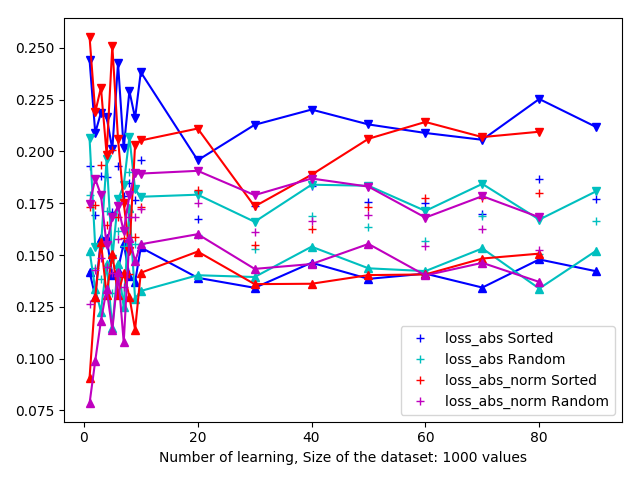
\includegraphics[height=\moyen]{sources/data/etfn/graph2.png}
	\caption{Variation d'aprensitssage en fonction du nombre d'aprentissage}
	\label{etfn2}
\end{figure}

On peut voir qu'a partir d'une vingtaine d'aprentissages, l'erreur stagne a une valeur moyenne
aux alentours des $0.175$ pour les données triées et
aux alentours des $0.15$ pour les données non triées.

Pour réduire cette erreur, il peut être bien de prendre la moyenne interquartiles, qui sera un bien meilleur indicateur.

\begin{figure}[H]
    \center
    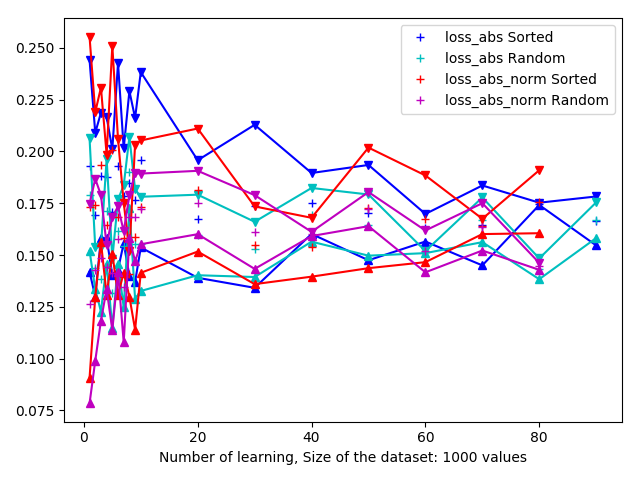
\includegraphics[height=\moyen]{sources/data/etfn/graph3.png}
	\caption{Variation interquartile d'aprensitssage en fonction du nombre d'aprentissage}
	\label{etfn3}
\end{figure}
\vspace{-5pt}
La Fig.\ref{etfn2} et la Fig.\ref{etfn3} n'ont pas de differences significatives...

\subsubsection*{L'après midi :}

Une base de donnée en ligne a été trouvée : \url{www.kaggle.com/harlfoxem/housesalesprediction}.
L'apres midi à été dédiée à coder un réseau qui tournera durant le WE affin de regresser ces données.
